\documentclass[11pt]{exam}

\usepackage{amsmath, amssymb, multicol}
\usepackage{graphicx}
\usepackage{textcomp}
\usepackage{tikz}

\def\d{\displaystyle}
\def\b{\mathbf}
\def\R{\mathbb{R}}
\def\Z{\mathbb{Z}}
\def\N{\mathbb{N}}
\def\pow{\mathcal{P}}
\def\st{~:~}
\def\bar{\overline}
\def\inv{^{-1}}
\def\imp{\rightarrow}
\def\and{\wedge}


%\pointname{pts}
\pointsinmargin
\marginpointname{pts}
\addpoints
\pagestyle{head}
%\printanswers

\firstpageheader{Math 228}{\bf Practice Problems 3: Functions}{Spring 2012}


\begin{document}
\noindent \textbf{Instructions}: The problems below are purely for you to practice.  I will not collect these, but it is still a good idea to write out your solutions in full.  Any of these problems or problems similar are fair game for quizzes and exams.  

\begin{questions}
\question Find all functions $f: \{1,2,3\}$ to $\{a,b\}$.  How many are there?  How many are one-to-one?  How many are onto?  How many are both?

\question Find all functions $f: \{1,2\}$ to $\{a,b,c\}$.  How many are there?  How many are one-to-one?  How many are onto?  How many are both?

\question Consider the function $f:\{1,2,3,4,5\} \to \{1,2,3,4\}$ given by the table below:

\begin{center}
\begin{tabular}{c||c|c|c|c|c}
              $x$ & 1 & 2 & 3 & 4 & 5 \\ \hline
              $f(x)$ & 3 & 2 & 4 & 1 & 2
            \end{tabular}
\end{center}

\begin{parts}

  \part Is $f$ one-to-one?  Explain.
  \part Is $f$ onto?  Explain.


\end{parts}

\question Consider the function $f:\{1,2,3,4\} \to \{1,2,3,4\}$ given by the graph below.
\begin{multicols}{2}
\begin{center}
  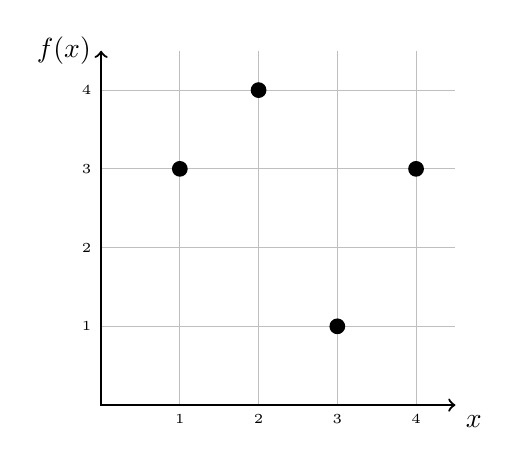
\begin{tikzpicture}[scale=1]
    \draw[thin, gray!50] (0,0) grid (4.5, 4.5);
    \draw[<->, thick] (0,4.5) node[left] {$f(x)$} -- (0,0) -- (4.5,0) node[below right] {$x$};
    \foreach \x in {1,2,3,4}
      \draw (\x,0) node[below] {\tiny \x} (0, \x) node[left] {\tiny \x};
    \fill (1,3) circle (.1) (2,4) circle (.1) (3,1) circle (.1) (4,3) circle (.1);
  \end{tikzpicture}
\end{center}



\begin{parts}
  \part Is $f$ one-to-one?  Explain.
  \part Is $f$ onto?  Explain.
\end{parts}

\end{multicols}


\question For each function given below, determine whether or not the function is one-to-one and whether or not the function is onto.
\begin{parts}
  \part $f:\N \to \N$ given by $f(n) = n+4$.
  \part $f:\Z \to \Z$ given by $f(n) = n+4$.
  \part $f:\Z \to \Z$ given by $f(n) = 5n - 8$.
  \part $f:\Z \to \Z$ given by $f(n) = \begin{cases}
                                         n/2 & \mbox{ if $n$ is even}\\
                                         (n+1)/2 & \mbox{ if $n$ is odd}.
                                       \end{cases}$
\end{parts}

\question Let $A = \{1,2,3,\ldots,10\}$.  Consider the function $f:\pow(A) \to \N$ given by $f(B) = |B|$.  So $f$ takes a subset of $A$ as an input and outputs the cardinality of that set.  
\begin{parts}
  \part Is $f$ one-to-one?  Prove your answer.
  \part Is $f$ onto?  Prove your answer.
  \part Find $f\inv(1)$.
  \part Find $f\inv(0)$.
  \part Find $f\inv(12)$.
\end{parts}

\question Let $A = \{n \in \N \st 0 \le n \le 999\}$ be the set of all numbers with three or fewer digits.  Define the function $f:A \to \N$ by $f(abc) = a+b+c$, where $a$, $b$, and $c$ are the digits of the number in $A$.  For example, $f(253) = 2 + 5 + 3 =  10$.
\begin{parts}
  \part Find $f\inv(3)$.
  \part Find $f\inv(28)$.
  \part Use one of the parts above to prove that $f$ is not one-to-one.
  \part Use one of the parts above to prove that $f$ is not onto.
\end{parts}

\question Find a set $X$ and a function $f:X \to \N$ so that $f\inv(0) \cup f\inv(1) = X$.

\question What can you deduce about the sets $X$ and $Y$ if you know,
\begin{parts}
  \part there is a one-to-one function $f:X \to Y$.  Explain.
  \part there is a onto function $f:X \to Y$.  Explain.
  \part there is a bijection $f:X \to Y$.  Explain.
\end{parts}

\question Suppose $f:X \to Y$ is a function.  Which of the following are possible?  Explain.
\begin{parts}
  \part $f$ is one-to-one but not onto.
  \part $f$ is onto but not one-to-one.
  \part $|X| = |Y|$ and $f$ is one-to-one but not onto.
  \part $|X| = |Y|$ and $f$ is onto but not one-to-one.
  \part $|X| = |Y|$, $X$ and $Y$ are finite, and $f$ is one-to-one but not onto.
  \part $|X| = |Y|$, $X$ and $Y$ are finite, and $f$ is onto but not one-to-one.
\end{parts}

\question Consider the function $f:\Z \to \Z$ given by $f(n) = \begin{cases}
                                                                 n+1 & \mbox{ if $n$ is even}\\
                                                                 n-3 & \mbox{ if $n$ is odd}.
                                                               \end{cases}$
\begin{parts}
  \part Is $f$ one-to-one?  Prove your answer.
  \part Is $f$ onto?  Prove your answer.
\end{parts}


\end{questions}




\end{document}


